Al saltar por primera vez a la tarea idle, nos aseguramos de tener inicializadas todas las TSS de las distintas tareas (2 por tarea, uno para la tarea en si y la otra para la bandera). La tarea inicial, desde donde se salta por primera vez a la idle, tambien debe tener un espacio pare el contexto de ejecucion, en donde el procesador guardara el estado del kernel para luego pasar a la ejecucion de tareas. La tarea idle debe ser mapeada sobre la memoria del kernel y compartir su CR3; ya que de no ser asi, y ubicarla en el mar con las demas, corremos el riesgo de que sea corrompida por otra tarea mediante un cañonazo, comprometendo la estabilidad del sistema.

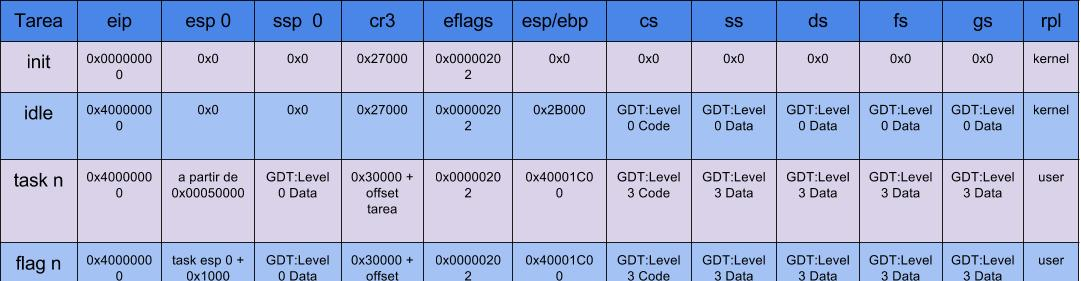
\includegraphics[scale=0.4]{diagramas/descriptoresDeTareas.jpg}
Mapeo en memoria del contexto de ejecucion de la tarea Idle y de las tareas.\\


Para que el procesador ubique la TSS de la tarea, incluimos en la GDT, por cada una, 2 entradas (tarea y bandera). Estas entradas son Descriptores de tarea, y le seteamos el limite minimo para las TSS que es de 0x67.

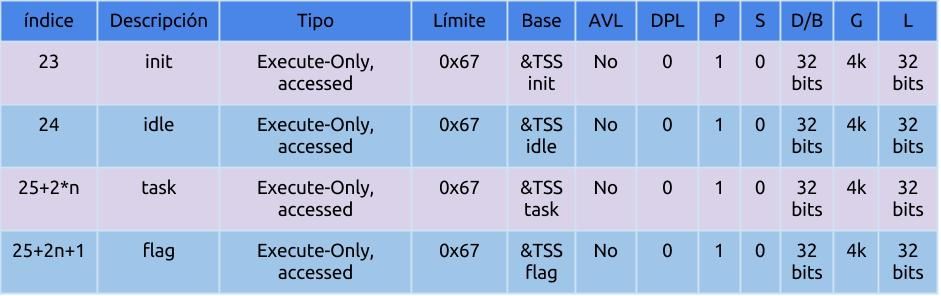
\includegraphics[scale=0.4]{diagramas/entradasGDTParaTareas.jpg}
Valores de las entradas de la GDT para la tarea Idle, Tareas y Banderas.\\



